%% !TeX encoding = UTF-8
%% !TeX program = pdflatex
%% !BIB program = bibtex
%%
%%% Um einen Artikel auf deutsch zu schreiben, genügt es die Klasse ohne
%%% Parameter zu laden.
\documentclass[biblatex]{lni}
\addbibresource{bibliographie.bib}
%%% To write an article in English, please use the option ``english'' in order
%%% to get the correct hyphenation patterns and terms.
%%% \documentclass[english]{class}
%%
\begin{document}
\include{listing}
%%% Mehrere Autoren werden durch \and voneinander getrennt.
%%% Die Fußnote enthält die Adresse sowie eine E-Mail-Adresse.
%%% Das optionale Argument (sofern angegeben) wird für die Kopfzeile verwendet.
\title[Infrastructure as Code]{Infrastructure as Code - Nutzen für und Integration in DevOps}
%%%\subtitle{Untertitel / Subtitle} % if needed
\author[Gabriel Sperling \and Reinhold Jooß]
{Gabriel Sperling\footnote{DHBW Stuttgart Campus Horb, Informatik, Florianstraße 15, 72160 Horb am Neckar, Deutschland \email{i20031@hb.dhbw-stuttgart.de}} \and
Reinhold Jooß\footnote{DHBW Stuttgart Campus Horb, Informatik, Florianstraße 15, 72160 Horb am Neckar, Deutschland
\email{i20016@hb.dhbw-stuttgart.de}}}
\startpage{1} % Beginn der Seitenzählung für diesen Beitrag / Start page
\editor{Prof. Dr.-Phil. Antonius van Hoof} % Names of Editors
\booktitle{Advanced Software-Engineering} % Name of book title
\year{2022}
%%%\lnidoi{18.18420/provided-by-editor-02} % if known
\maketitle

\begin{abstract}
Im Umfang dieser Arbeit wird die Ausübung von Infrastructure as Code beleuchtet und wie diese zu einer effizienteren Softwareentwicklung führen kann. Dem Leser werden die Grundlagen von IaC und dessen Prinzipien nähergebracht. Dadurch werden die Vorteile im Gegensatz zu einer manuellen Konfiguration verdeutlicht. Außerdem werden die Anwendungsbereiche von IaC untersucht. Innerhalb dieser Ausarbeitung werden des Weiteren die Risiken welche während der Arbeit mit IaC auftreten können, dargelegt und anschließend erläutert wie das Eintreten dieser vorgebeugt werden kann. Eine Integration von IaC in Softwareentwicklung wird ebenfalls betrachtet und mit Hilfe des Softwaretools Ansible in einem Anwendungsbeispiel näher beleuchtet. Im Gesamten soll der Nutzen von Infrastructure as Code in DevOps verdeutlicht werden. Dabei soll diese Arbeit Aufklärung darüber schaffen wie es am besten eingesetzt wird und was es bei dessen Nutzung zu beachten gilt.
\end{abstract}
\begin{keywords}
Infrastructure as Code \and DevOps \and Cloud Age %Keyword1 \and Keyword2
\end{keywords}
%%% Beginn des Artikeltexts
\section{Probleme der manuellen Konfiguration als Motivation für IaC} %\textcolor{red}{ANPASSEN ZU MOTIVATION ABER HOW}}
Dieser Abschnitt soll aufzeigen, welche Komplikationen und Hindernisse entstehen, sollte eine Infrastruktur manuell konfiguriert werden. Dadurch können neben den Risiken, welche dies für ein System mit sich bringt, auch weitere Vorteile einer automatisierten Konfiguration aufgezeigt werden und so eine Einleitung in den Nutzen von IaC gegeben werden. 

Die Motivation, DevOps und IaC in die interne Infrastruktur zu integrieren, geht aus den Schwächen einer manuellen Konfiguration der IT-Infrastruktur hervor. Für ein Unternehmen ist es von großer Bedeutung eine stabile und leistungsstarke Umgebung für ihre Mitarbeiter und Software zu bieten. Durch hohe Qualität der Infrastruktur können Arbeitsprozesse effizienter durchgeführt und das Aufkommen von Fehlern und entstehenden Schäden verringert werden. Dementsprechend wird beim Aufbau der Infrastruktur ein großes Augenmerk auf die Zusammenstellung der Hardwarekomponenten gelegt. Die Anforderungen an die entstehende Recheneinheit müssen exakt definiert werden, um anschließend die benötigten Komponenten zusammestellen und installieren zu können. Sobald die Infrastruktur aufgebaut wurde, sollte diese dementsprechend ihren Zweck erfüllen, ohne dass in naher Zukunft mit Änderungen zu rechnen ist. Aufgrund von kontinuierlichen Änderungen in der Umgebung sind Überarbeitungen oder Erweiterungen der Infrastruktur jedoch beinahe unvermeidbar. Sobald diese auftreten muss vorerst erneut eine Planung stattfinden um den Änderungen gerecht zu werden, was einen hohen Ressourcenaufwand mit sich bringt. Die manuelle Konfiguration wird daher grundsätzlich zwar als stabile, jedoch sehr unflexible und kostenintensive Verwaltungsform betrachtet. Heutzutage wird dies als ein Hindernis betrachtet, da ein modernes Software-Engineering auf kurzschrittige und regelmäßige Releases abzielt, um eine erhöhte Flexibilität beim Implementierungsvorgang zu erreichen. Mit Hilfe von IaC soll daher eine automatische Konfiguration ermöglicht werden, um den Arbeitsaufwand für die Verwaltung der Infrastruktur zu verringern und damit für effizientere Releases im Software-Engineering zu sorgen.

Die Verringerung des Arbeitsaufwands kann anhand eines Beispiels verdeutlicht werden. Angenommen ein Unternehmen besitzt eine hohe Anzahl an verschiedenen Tochtergesellschaften, deren Webseiten über den Mutterkonzern geregelt werden. Sollte eine manuelle Konfiguration angewandt werden, muss vorerst ein leistungsstarker Server aufgebaut werden, welcher den Workload aller Tochtergesellschaften verarbeiten kann. Des Weiteren müssen anschließend die jeweiligen virtuellen Maschinen für die einzelnen Tochtergesellschaften vollständig aufgebaut und eingerichtet werden. Durch das Nutzen von Infrastructure as Code hätte ein Definieren einer VM als Code die Automatisierung der VM-Erstellung für die Tochtergesellschaften ermöglicht. Für identische Server hätte eine einzelne Definition des gewünschten Servers gereicht. Anschließend kann durch eine Automations-Software anhand der Definition eine beliebte Menge an Servern erstellt werden, welcher der Definition entsprechen. Falls nun bei einer der Tochtergesellschaften eine erhöhte Anzahl an Kunden auf deren Webseite festgestellt wird, wäre es möglicherweise notwendig die Speicherkapazität der VM zu erhöhen. Manuell müsste eine neue Festplatte eingebaut und auf dem Server konfiguriert werden. Anschließend muss sie der VM zugewiesen werden. Mit IaC könnte dieser Vorgang beschleunigt werden, indem die Speicherkapazität im Code als ein Parameter definiert wird, welcher beliebig angepasst werden kann. Der gesamte Overhead, welcher von Beginn an durch das Erwerben und Aufbauen der entsprechender Hardware entsteht, würde verfallen beim Anwenden von IaC. Grund hierfür ist das Umsteigen auf cloudbasierte Dienste diverser Anbietern in der heutigen Zeit. Ressourcen wie Speicherplatz, Arbeitsspeicher oder CPUs können beliebig zusammengestellt und eingesetzt werden um eine Infrastruktur zu generieren und zu erweitern.
Die Vorteile einer Nutzung von IaC gegenüber einer manuellen Konfiguration werden in Abbildung \ref{fig:manualvsca} verdeutlicht. 
\pagebreak
\begin{figure}
    \centering
    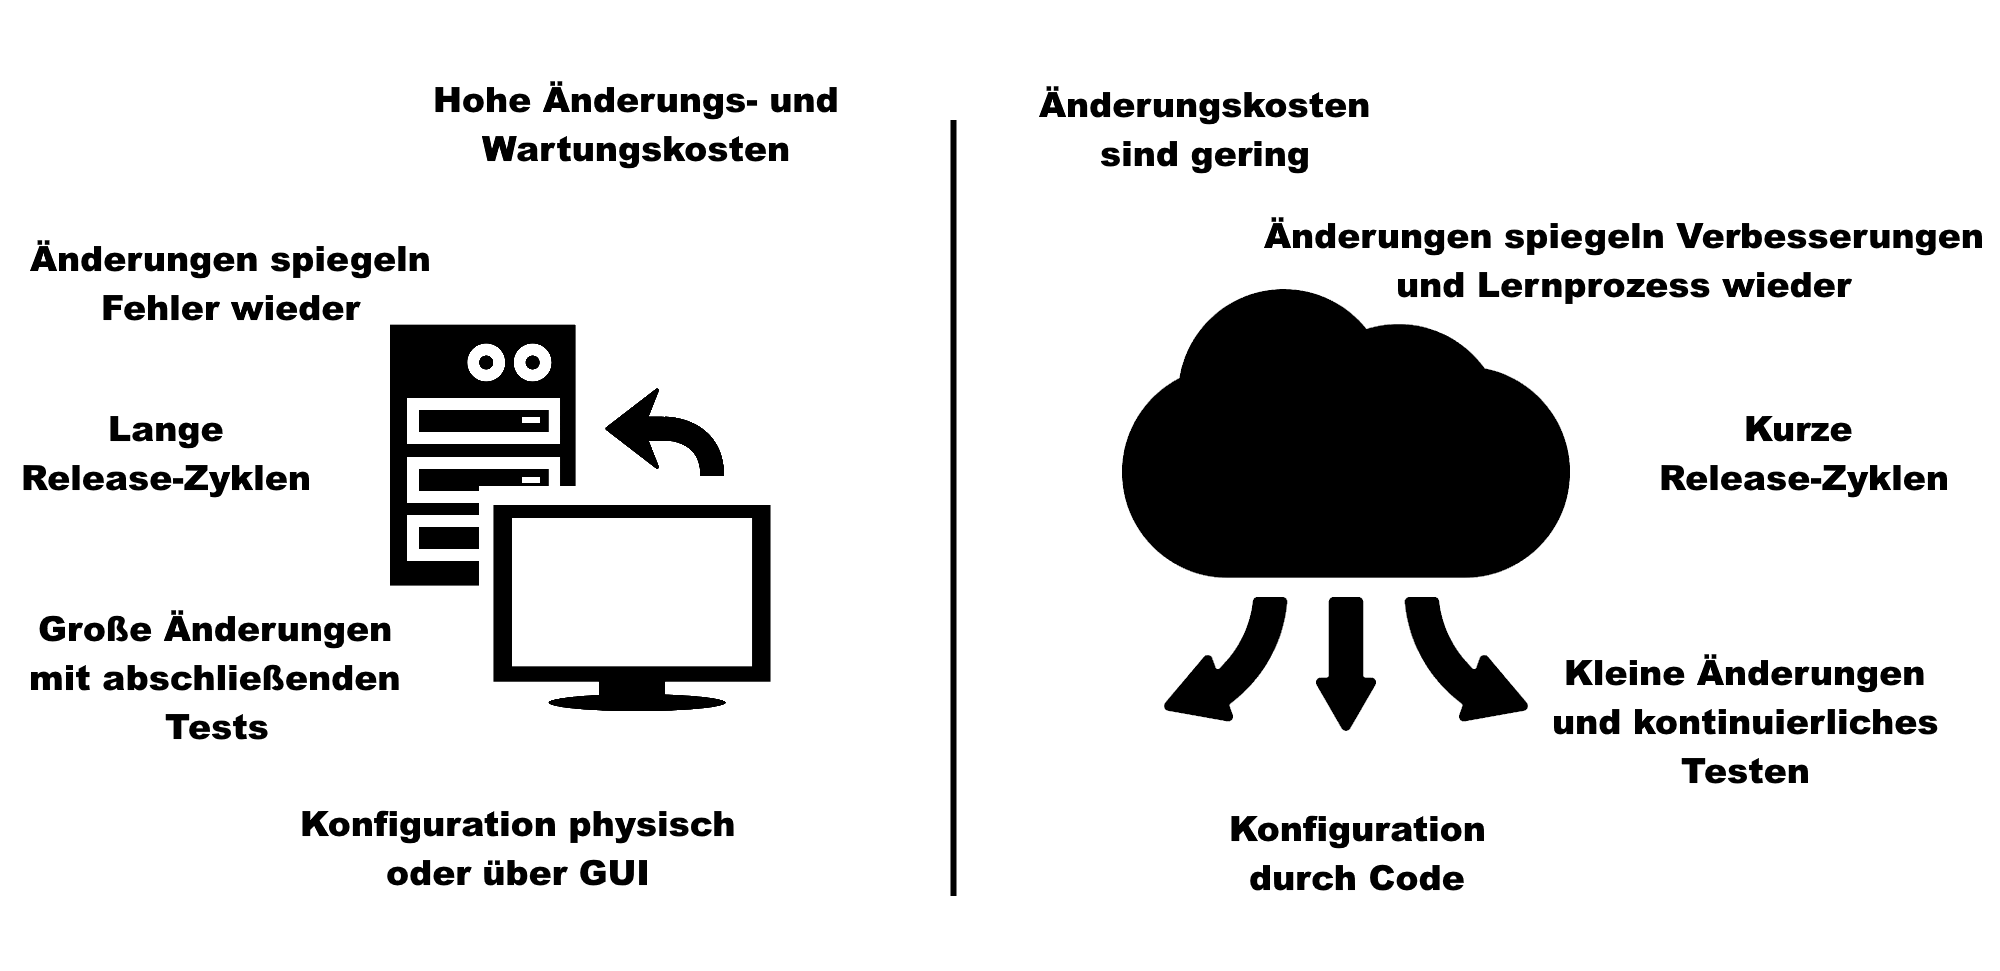
\includegraphics[width=12cm]{iac.png}
    \caption{Manuelle Konfiguration und Konfiguration in der Cloud Age im Vergleich \cite{Morris.December2020}}
    \label{fig:manualvsca}
\end{figure}\\

% \newpage
\section{Grundlagen von IaC}
In diesem Abschnitt soll dem Leser ein Einblick in die Grundlagen von IaC gegeben werden. Dabei wird vermittelt aus welchen Umständen IaC entstand und wieso dieses angewandt wird. Dafür werden verschiedenen Prinzipien betrachtet, die es beim Erstellen der Infrastruktur zu beachtend gilt. Abschließend werden die verschiedenen Bestandteile der Infrastruktur, welche sich später mit IaC definieren lassen aufgezeigt.
\subsection{Einführung in IaC}
Auf Grund einer stetigen Nachfrage nach schnellen und regelmäßigen Software-Realeases und der Entwicklung komplexer werdenden Systeme existieren mittlerweile viele technische und organisatorische Praktiken um die Herausforderungen des modernen Markts der Softwareentwicklung zu befriedigen. Diese Praktiken werden unter dem Begriff \textquote{DevOps} zusammengefasst und versuchen die Softwareentwicklung (\textbf{Dev}elopment) mit den Aufgaben der IT (IT-\textbf{Op}erations) zu kombinieren. Unter diese Praktiken fällt auch Infrastructure as Code \cite[S. 580-581]{Guerriero.2019}.

Infrastructure as Code ist ein relatives junges Konzept der Informatik, welches aus komplexen Anforderungen der \textquote{Cloud Age} (Bereitstellung von virtuellen Ressourcen über die Cloud) hervorkam. Durch die in der Cloud vorhandene Vielzahl an Ressourcen ergaben sich verschiedenste Anforderungen im Bereich der Verwaltung. Die verwendeten Ressourcen innerhalb eines Unternehmens welche die Infrastruktur zusammenstellten wurden in der \textquote{Iron Age} (physische Hardware zum Aufbau eines Systems) manuell konfiguriert und erstellt. Somit war es möglich die Infrastruktur gezielt auf den Anwendungsbereich zu spezifizieren und anzufertigen. Auf einen genauen Aufbau, hohe Stabilität und eine Gesamtheit der Struktur wurde somit großen Wert gelegt. Grund hierfür sind die hohen Kosten die eine Änderung der Struktur mit sich bringt. Im Umkehrschluss führt dies wiederum zur Gefahr zukünftige Änderungen des Systems mit einem hohen Aufwand zu verbinden. So kann es in extremen Fällen beispielsweise vonnöten sein, das komplette System aufgrund des rückständigen Zustands komplett abzubauen, um es zu erneuern. In der modernen Zeit wurde dieses Risiko deutlich verringert. Durch die Cloud Age sind die Kosten zur Bereitstellung und Änderung der Infrastruktur mit nur sehr geringem Aufwand verbunden, da die Ressourcen nicht mehr physisch sondern virtuell gegeben sind. Jedoch brachte diese Änderung der Technologie nicht direkt eine Vereinfachung der Systemverwaltung mit sich \cite{Morris.December2020}. Da sich eine Systemverwaltung der Cloud Age fundamental von einer in der Iron Age unterscheidet, muss die Arbeitsweise mit dieser angepasst werden, um ein optimales Vorgehen zu erreichen. Die geringen Kosten und Einfachheit kleiner Änderungen können in der Cloud Age ausgenutzt werden um eine erhöhte Qualität in geringer Zeit zu erreichen.
\subsection{Eigenschaften und Prinzipien beim Arbeiten mit IaC}
Mit Hilfe von IaC soll das Vorgehen die Infrastruktur zu verwalten vereinfacht und automatisiert werden. Sie ist eine Möglichkeit neue Zusätze an die Infrastruktur schnell auszuliefern, Änderungen einfach vorzunehmen und ein durch diese entstehendes Risiko zu verringern. Verwendete Tools in der Entwicklung und von weiteren Teilnehmern des Betriebs werden vereinheitlicht und die entstehenden Systeme möglichst sicher und effizient gestaltet, um später eine qualitativ hochwertige Verwaltung zu erlangen. Dabei ist es wichtig einen Fokus auf die Vorteile der Cloud Age, mit Hilfe verschiedener Core Practices und Prinzipien zu legen. Dazu gehört die gesamte Infrastruktur als Code zu definieren, um eine Wiederverwendbarkeit der Ressourcen zu garantieren, diese konsistent zu halten und eine möglichst hohe Transparenz für die Anwender zu generieren. Dafür wird zumeist eine deklarative Programmiersprache verwendet, wodurch der Code einen hohen Informationsanteil über die erstellte Systemressource liefert. Des Weiteren ist es wichtig den erstellten Code ständig zu testen und anschließend auszuliefern. Durch eine Integration neuer Änderungen, die im Laufe der Entwicklung getestet wird, können in geringeren Zeitabständen Erweiterungen ausgeliefert werden. Dadurch kann die Qualität des Endprodukts von Beginn an entwickelt werden, entgegengesetzt zum späteren Testen, in welchem die Qualität vielmehr \glqq hineingetestet\grqq{} wird. Damit korrespondierend ist es Änderungen und Bestandteile klein und isoliert zu halten. Neben einer besseren Übersicht und Verständnis des Codes, wird somit für ein stabiles System gesorgt, welches bei Änderungen nicht leicht zerfällt. Wie unschwer zu erkennen ist, ähneln diese Praktiken dem Vorgehen, welches im Bereich des Software-Engineerings angewandt wird. Die verschiedenen Prinzipien welche beim Anwenden von IaC empfohlen werden besitzen eine ähnliche Affinität. So ist es von großer Wichtigkeit das zu entstehende System reproduzierbar zu gestalten. Dadurch ist das System bei Fehlerfällen problemlos wiederherzustellen. Damit geht einher das Testen und die Reproduzierbarkeit dieser Tests konsistent zu halten und ebenso eine Replikation desselben Systems mühelos vorzunehmen. Im Falle von einer Verteilung mehrerer Systeme an verschiedene Verbraucher kann durch die Reproduzierbarkeit des Systems eine schnelle Auslieferung geschehen. Sobald eine Infrastruktur als Code definiert wurde sollte eine simple Reproduktion des Systems möglich sein, was dem Anwender enorme Freiheiten beim Erstellen, wie auch beim Löschen einer Infrastruktur gibt. Dadurch können die Risiken durch unvorhergesehen Fehler geschwächt werden. Ein weiteres Vorgehen welches sich einen Nutzen aus der schnellen und dynamischen Änderung von IaC macht sind es eben diese Fehler in Kauf zu nehmen. Da durch IaC eine Beachtung von Fehlern nicht so ausschlaggebend ist wie bei manuellen Systemen, ist es von umso größerer Bedeutung, die zu definierenden Systeme als unzuverlässig zu betrachten und mit Fehlern zu rechnen. Ein Austausch des Systems, sollte dieses den Anforderungen ungenügend sein oder das Ersetzen eines unbrauchbaren Systems, aufgrund von Ausfällen oder Fehlern muss unbedingt in der Herstellung bedacht werden. Daraus folgend muss das System für eine ununterbrochene Laufzeit sorgen. Sollte eine Ressource ausfallen, kann das System durch das schnelle Ausliefern einer neuen Instanz der Ressource gerettet werden. Damit kommen wir zum nächsten Prinzip, der Verwerfbarkeit von zu erstellenden Infrastrukturteilen. Es ist wichtig sich klarzumachen, wie dynamisch haltbar ein System durch die Virtualisierung in der Cloud Age ist. Die einzelnen Bestandteile sollten daher nicht als unerlässlich, sondern viel eher als entbehrbar betrachtet werden. Wird die Infrastruktur entsprechend designt, wird dem Anwender weitergehend Freiheit gewährt, dieses jederzeit neuzuformen, ohne die zu leistende Arbeit des Systems zu unterbrechen. Die einzelnen Bestandteile sollten dementsprechend möglichst minimal gestaltet werden, um Komplikationen, welche durch eine weite Variation der Bestandteile entstehen könnte, zu verhindern. Der Verwaltungsaufwand steigt nicht nur mit der Anzahl an Bestandsteilen sondern auch mit deren verschiedenen Typen. Um den Aufwand möglichst gering zu halten, sollte daher mit einer möglichst geringen Anzahl an Typbestandteilen gearbeitet werden, da es beispielsweise leichter ist eine Vielzahl an identischen Servern zu handhaben, als eine geringe Anzahl vollkommen verschiedener Server. Hiermit wird wiederum das oben genannte Prinzip der Reproduzierbarkeit betont, welches dieses Vorgehen weitergehend ergänzt \cite{Morris.December2020}.

Ein weiteres zu befolgendes Prinzip, ist die einheitliche Entwicklung des Systems. Das zukünftige Arbeiten wird unumgänglich eine Erweiterung des bestehenden Systems mit sich bringen. Dabei besteht die Gefahr das System durch ad hoc Änderungen weniger flexibel zu machen, da verschiedene Bestandteile mit ihrer ursprünglichen Aufgabe verfremdet werden. Die erfolgenden Erweiterungen sollten daher ebenfalls über den Code definiert und somit parametrisiert werden. Wiederum entsteht dadurch die Notwendigkeit alle Prozesse, die beim Verändern des Systems durchgeführt werden, zu automatisieren. Prinzipiell ist es gewünscht alle vorzunehmenden Prozesse reproduzierbar zu gestalten. Sollte eine Änderung on-the-fly vorgenommen werden besteht die bereits genannte Gefahr einer Inkonsistenz durch Verlust an Flexibilität, welche bei zukünftigen Anpassungen des Systems wiederum zu Fehlern führen können. Zwar sollten sich diese Fehler durch den einfachen Austausch der Ressource beheben lassen, können jedoch beispielsweise für einen unerwünschten Ausfall des Systems oder Teile dessen führen. Eine Lösung können z.B. Skripts liefern, welche zur Konfiguration beisteuern. Dadurch wird gewährleistet das gleiche Vorgehen beim Konfigurieren einer Ressource vorzunehmen. 
\subsection{Aufbau einer Infrastruktur}
Da nun die verschiedenen Punkte, welche beim Erstellen der Infrastruktur zu beachten sind, erläutert wurden, gilt es zu klären, welche Bestandteile der Infrastruktur angehören. Generell können diese in drei Kategorien unterteilt werden.
\begin{itemize}
    \item Anwendungen (z.B. Anwendungspakete, Containerinstanzen)
    \item Laufzeitplattformen für Anwendungen (z.B. Server, Container Cluster, Datenbank Cluster)
    \item Infrastrukturplattformen (z.B. Recheneinheiten, Netzwerkstrukturen, Speicher)
\end{itemize}
Diese drei Kategorien können für ein besseres Verständnis als Schichtenmodell angesehen werden, welche sich gegenseitig ergänzen. Die Anwendungen stellen dabei die oberste Ebene der Struktur dar. Sie stellen dem Anwender die benötigten Werkzeuge für die gewünschte Arbeitsumgebung zur Verfügung. Geregelt werden diese in der Laufzeitplattform für Anwendungen. Hier können Konfigurationen vorgenommen werden, um die Anwendung mit verschiedenen Services und Berechtigungen auszustatten, so z.B. der Anbindung an eine Datenbank. Als unterste Ebene kann die Plattform für die Infrastruktur gesehen werden. In dieser werden die grundlegenden Ressourcen, welche zur Auführung der einzelnen Bestandteile benötigt werden, bereitgestellt. Dazu gehören unter anderem Rechenressourcen, wie Virtual Machines oder auch Server und Container. Des Weiteren werden hier Speicherressourcen eingerichtet, welche in verschiedenen Formen bereitgestellt werden können. Beispielsweise Blockspeicher durch eine Virtualisierung von Partitionen, Dateisysteme auf einem Netzlaufwerk oder auch Objektspeicher in einer spezifischen Ausführung. Dabei können die Speichereinheiten natürlich gezielt auf die Anwendungsbereiche verteilt werden, z.B. für einen dedizierten Server oder verschiedene Container. Zuletzt werden in dieser Schicht auch verschiedene Netzwerkressourcen betrachtet. Somit können für die Anwendung nötige Gateways, Routing oder auch VPNs konfiguriert werden. Damit verbunden sind somit auch Proxys, sowie Netzwerkadressen oder DNS Einträge.

Für die Umsetzung von IaC gibt es zwei unterschiedliche Lösungsansätze. Hierbei wird zwischen statischer und dynamischer IaC unterschieden. Statische IaC-Lösungen stellen hierbei den traditionellen Lösungsweg dar. Hierbei werden Skripts erstellt und die Konfiguration wird auf die Infrastruktur einmal angewendet. Diese Infrastruktur ändert sich hierbei nicht, sofern das erstellte Skript nicht erneut angewendet wird, unabhängig davon ob das Skript manuell oder automatisiert durch eine Pipeline ausgeführt wird. Auf der anderen Seite befinden sich die dynamischen IaC-Lösungen, die aktuell weiterentwickelt werden und damit statische Lösungen erweitern sollen. Das Prinzip dahinter beruht auf externen Signalen, von denen Teile der Skripts abhängen. Die Infrastruktur wird automatisch auf die ändernden Signale angepasst und wieder neu angewendet. Beispielsweise kann eine Infrastruktur in Abhängigkeit von der Last konfiguriert sein, sodass diese bei steigender oder sinkender Auslastung dementsprechend Ressourcen zur Verfügung stellt oder freigibt. Dies ist besonders vorteilhaft für eine sogenannte \textquote{pay-per-use} Infrastruktur in beispielsweise einer Cloud. Im Gegensatz dazu ist es möglich diese Funktionalität durch eine Pipeline auf eine statische Lösung anzuwenden, jedoch wird dadurch der dynamische Aspekt ausgelagert, was unter anderem zu weiterem Aufwand führt. Dadurch wird es schwerer das gesamte System zu testen und zu analysieren, weshalb der dynamische Ansatz vorzuziehen ist. Jedoch wird damit auch eine robustere und automatisierte Lösung zum Testen der dynamisch implementierten Infrastruktur benötigt \cite{Sokolowski.2022}.

Zu guter Letzt, wird in diesem Kapitel TOSCA (Topology and Orchestration Specification for Cloud Applications) kurz beschrieben. TOSCA stellt einen Standard für das Design von Infrastrukturen dar, der aktuell entwickelt und erforscht wird. Hierbei wird die Infrastruktur durch einen Graph visualisiert, der aus wiederverwendbaren Knoten und Kanten besteht. Dafür werden die Knoten und Beziehungen kategorisiert, um einfache Bausteine für die Entwicklung der Infrastruktur zur Verfügung zu stellen. Dabei bieten Plattformen, die den Standard implementieren bereits unterschiedliche Bausteine für bestimmte Anwendungen an, wie beispielsweise MySQL \cite{Artac.2017}. Ein solcher Standard ist hilfreich, um die Kompatibilität von unterschiedlichen Plattformen und Werkzeugen für IaC zu verbessern. Dadurch werden neue Möglichkeiten in der Orchestrierung von Infrastruktur offengelegt und komplexere Strukturen werden ermöglicht.

\begin{figure}
    \centering
    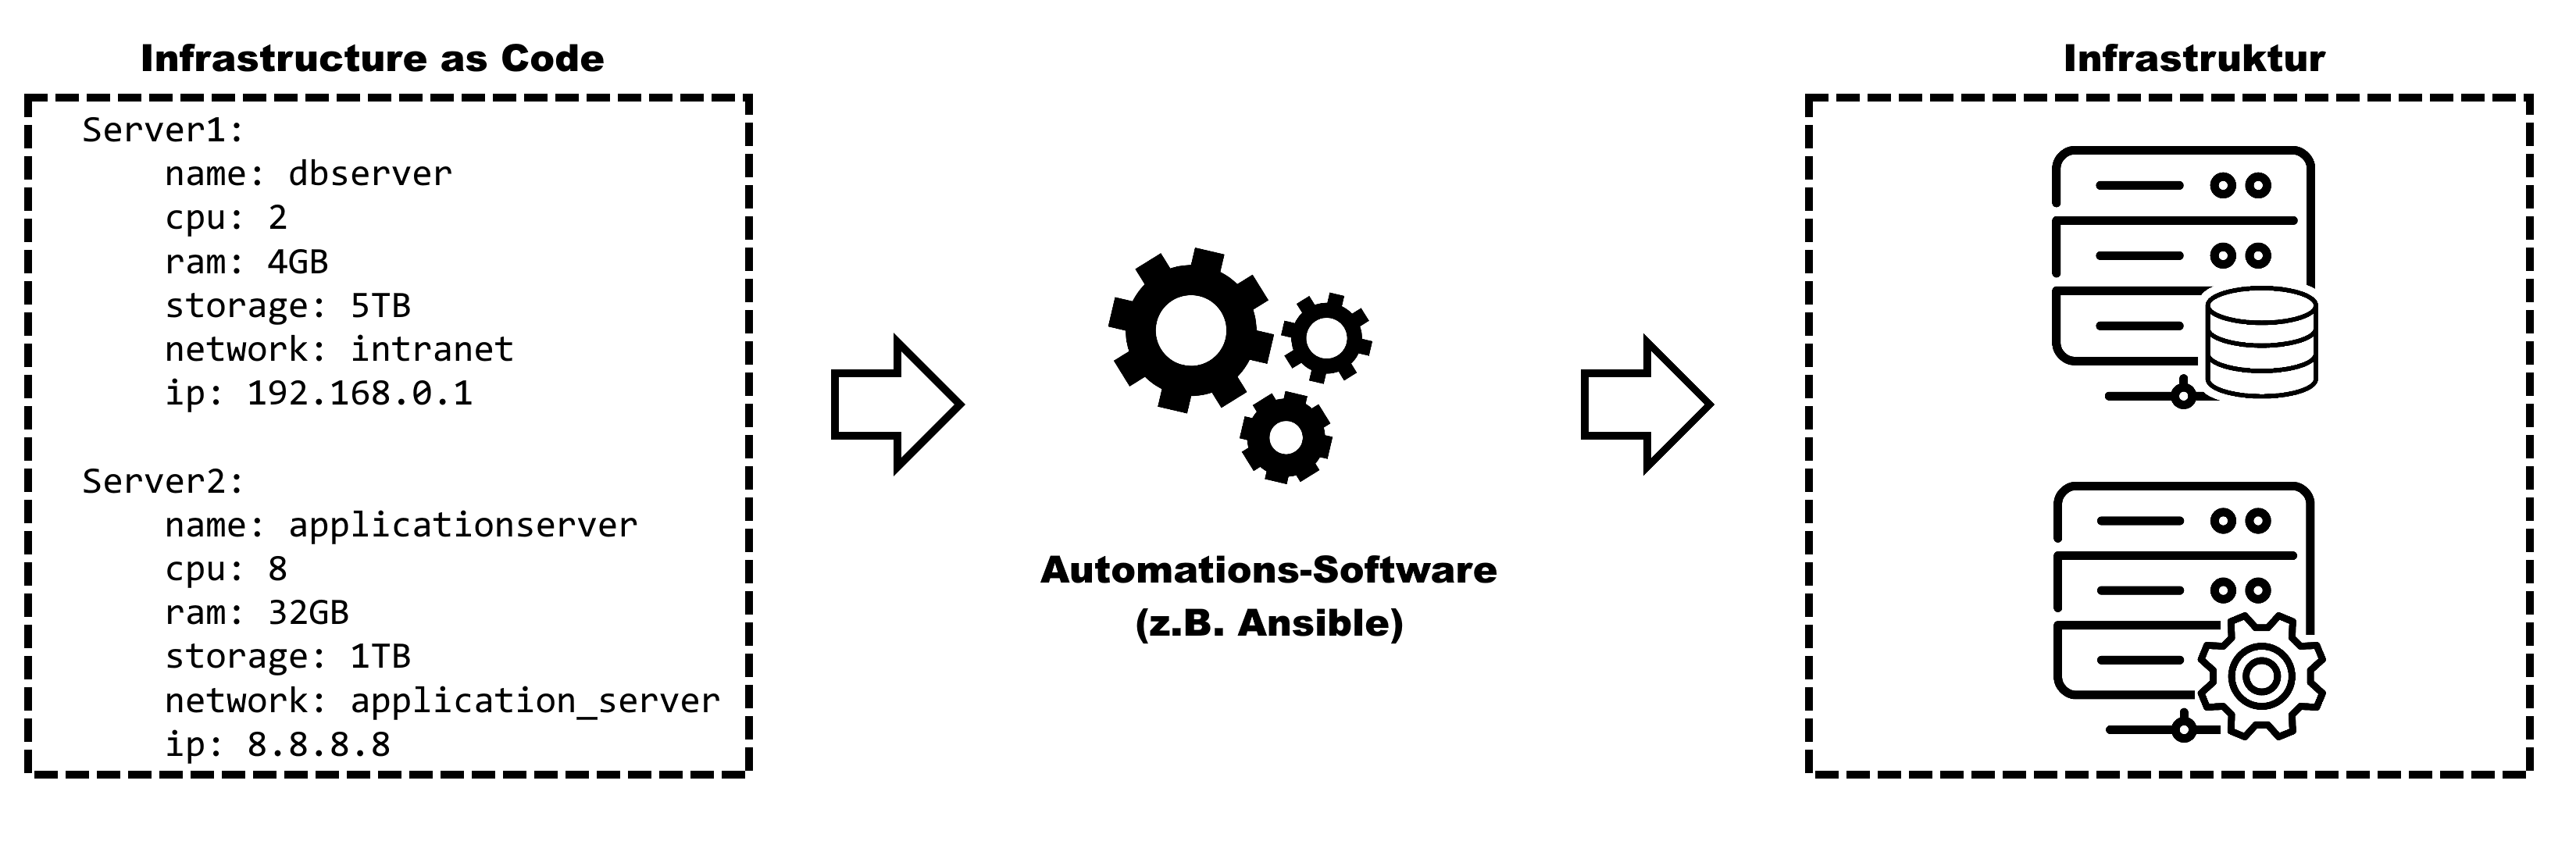
\includegraphics[width=12cm]{iac-scheme.png}
    \caption{IaC zur automatisierten Erstellung der Infrastruktur}
    \label{fig:iacschemata}
\end{figure}

% \newpage
\section{Nutzen und Vorteile von IaC}
Um den Nutzen von IaC zu verdeutlichen, können verschiedene Argumente gegen die Einführung von IaC betrachtet werden, welche \cite{Morris.December2020} hervorhob. Diese können durch die entstehenden Vorteile bei einer frühzeitigen Anwendung von IaC entkräftet werden. 

\textbf{Gegenargument: Eine Automatisierung von Änderungen bringt keinen ausreichenden Mehrwert bei einer geringen Anzahl an Änderungen.}\\
Beim Planen der Infrastruktur wird vorzugsweise davon ausgegangen das System einmal zu erschaffen und es anschließend als finalisiert zu betrachten und es somit zukünftig nicht mehr entscheidend anzupassen. Objektiv gesehen bleiben Systeme jedoch in den wenigstens Fällen auf den anfangs festgelegten Nutzen beschränkt und werden stetig erweitert. Beispielsweise könnte durch ein Betriebssystem-Update die Notwendigkeit entstehen dutzende Server zu aktualisieren. Durch eine Automatisierung mit IaC wären diese Änderungen innerhalb kürzester Zeit erledigt. Vor allem in der Cloud Age profitieren Anwender von vielen Änderungen, um ihre Systeme stabiler zu machen. Eine Automatisierung der Infrastruktur bringt daher mehr Vorteile, als ein System durch viele manuelle Anpassungen instabil werden zu lassen.   

\textbf{Gegenargument: Es sollte zuerst gebuilded und anschließend automatisiert werden.}\\
IaC anzuwenden zeigt zu Beginn einer Systemerstellung einen sehr hohen Arbeitsaufwand, da vorerst alle Ressourcen definiert werden müssen, bevor diese tatsächlich erstellt werden können. Meist wird daher als schnellere Alternative ein neues cloudbasiertes System manuell erstellt, mit der Absicht dessen Automatisierung später hinzuzufügen. Dadurch entstehen grundsätzlich drei Probleme. Erstens werden viele der Vorteile einer Automatisierung nicht umgesetzt. Eine schnelle Verteilung der benötigten Systeme kann nicht durchgeführt werden, nachdem ein System bereits größtenteils aufgebaut wurde. Zweitens können Tests leichter erstellt und direkt in die Automatisierung eingebunden werden. Dadurch kann beim ersten Aufbau der Infrastruktur bereits eine schnelle Fehlerbehebung stattfinden und ein Rebuild bei Problemen vorgenommen werden. Als letzter Punkt kann festgestellt werden, dass die Automatisierung bestehender Systeme ein sehr komplexes Vorhaben ist. Die bestehende Infrastruktur muss möglicherweise angepasst und erweitert werden. Aufgrund der Probleme sollte die Automatisierung bereits zu Beginn und während des Aufbaus einer Infrastruktur betrachtet werden. Durch IaC wird ein solches Vorgehen gewährleistet.

\textbf{Gegenargument: Es muss sich zwischen Schnelligkeit und Qualität entschieden werden.}\\
Es besteht grundsätzlich die Annahme bei der Bearbeitung einer Aufgabe die Qualität des Produkts und die Schnelligkeit der Erstellung in einen relativen Vergleich stellen zu müssen. Es kann keine hohe Qualität gewährleistet werden, wenn die Erstellung des Systems möglichst schnell ausgeführt werden muss. Dementsprechend kann kein qualitativ hochwertiges und stabiles System erstellt werden, wenn kein großer Zeitraum dafür verwendet wird. Wie sich laut \cite{Humble.2018} herausstellt ist diese Annahme jedoch falsch. Teams, welchen die Prinzipien der agilen Verfahren aus dem Software-Engineering Bereich bewusst sind, schaffen es demnach auch durch schnelle Releases ein hohe Qualität aufzuzeigen. Dieses Methodik kann auf IaC übertragen werden, um somit eine stabile Infrastruktur zu erschaffen, welche einen Fokus auf Schnelligkeit sowie Qualität legt. % Dadurch werden fortgehend auch die Schwächen durch ein

\section{Integration von IaC in Softwareentwicklung}
Nachdem nun der Nutzen und die Vorteile von Infrastructure as Code aufgezeigt wurden, geht es weiter mit dem praktischen Teil von IaC: Die Integration von IaC in der Softwareentwicklung. Hierbei gibt es drei verschiedene und wichtige Methoden, die bei der Integration zu beachten sind, die im Weiteren genauer erläutert werden: Neben dem Konzept, dass die gesamte Infrastruktur als Code definiert wird, ist es wichtig diese in kleine Teile zu unterteilen und den definierten Code kontinuierlich zu testen.

Weiterhin werden in diesem Kapitel sogenannte \textquote{Bad} und \textquote{Best} Practices für die Implementierung von Infrastructure as Code dargestellt. Damit wird ein Überblick darüber gegeben, was zu beachten ist und wie es richtig gemacht wird.

Zu Letzt wird knapp zusammengefasst, welche Tools für die Umsetzung von IaC genutzt werden. Hierbei wird insbesondere auch darauf eingegangen, was bei der Verwendung dieser Tools zu beachten ist.

Die erste der drei wichtigsten Methoden, welche bei der Integration von IaC zu beachten sind, beschäftigt sich mit den Überlegungen, was alles als Code definiert werden sollte. Offensichtlich ist es am besten jegliche Bestandteile der Infrastruktur in Code zu formulieren, da es dadurch theoretisch möglich wird die Prozesse um jede einzelne Komponente zu automatisieren. Praktisch ist dies jedoch nicht umsetzbar, weswegen es essentiell ist die wichtigsten Bestandteile zu identifizieren und diese bestmöglich zu definieren. Dazu gehören unter anderem der sogenannte \textquote{infrastructure stack}. Dieser beinhaltet alle Elemente, die über eine Cloud Plattform bereitgestellt werden können, die für die Softwareentwicklung notwendig sind. Außerdem sollen Abbildungen von Servern als Code definiert werden, da hierdurch das mehrfache Aufsetzen von Servern erleichtert und automatisiert wird. Ebenso sollten jegliche wiederverwendbare Konfigurationen in IaC-Skripts definiert werden, wie beispielsweise Server-Konfigurationen, die Anwendungen, Benutzer und notwendige Dateien enthalten. Wenn nun der bestmögliche Teil der Infrastruktur in Code definiert wurde, müssen die entstandenen Dateien in einem geeigneten System oder geeigneter Anwendung verwaltet werden. Diese entsprechen nicht den Tools, die für das Deployen der Skripts zuständig ist. Beispiel hierfür sind Version Control Systems, wie Git. 

Der Code wird entweder in einer deklarativen Sprache oder imperativen Sprache geschrieben. Deklarative Sprache haben den Vorteil, dass sie nützlich für die Definition des gewünschten Endzustands einer Komponente sind. Hiermit können übliche Konfigurationen einfach und konsistent verwendet werden. Auf der anderen Seite stehen imperative Sprachen, die flexibler sind. Mit dem imperativen Ansatz ist es möglich Variablen einzubauen, die die Infrastruktur auf eine bestimmte Situation anpasst, wobei der Code wiederverwendet wird und nicht für jeden Fall neu geschrieben werden muss \cite{Morris.December2020}. Deshalb ist es notwendig für den jeweiligen Use Case abzuwägen, welche Art der Sprache am besten geeignet ist. Es ist auch möglich beide Sprachen durch die Verwendung verschiedener Tools zu mischen, wobei dies mit Vorsicht zu genießen ist. Ebenso stellen die richtige Auswahl der Komponenten und Systeme eine große Rolle, wie auch die Auswahl eines geeigneten Version Control Systems. 

Jetzt wo der Code erstellt ist, beschäftigt sich die zweite Methode mit dem Testen des Codes. Das Ziel nach dem sich gerichtet werden kann besteht hierbei, dass der Code immer auf die Struktur erfolgreich anwendbar sein soll. Die wichtigsten Dinge, die getestet werden sollten sind, dass der Code die Infrastruktur in der gewollten Konfiguration hinterlässt, dass die Leistung und Sicherheit der Infrastruktur den Anforderungen entspricht und dass der Code überhaupt anwendbar ist. Ein Problem stellen hier Tests für deklarativen Code dar, da diese Tests bei jeder Änderung des Codes auch geändert werden müssen und damit wenig Nutzen und viel Aufwand haben. Progressive Testing stellt im Allgemeinen eine gute Methode zum Testen dar. Dabei werden schnelle und einfache Tests zuerst durchlaufen, die dann auf komplexeren und aufwändigeren Tests aufbauen. So können grobe Fehler früher entdeckt und durch einfache Tests besser aufgedeckt werden. Eine Pipeline zu verwenden ist empfehlenswert, da dadurch der Testprozess automatisiert und mit dem Deployment verbunden werden kann. Für jede Änderung können dann die Tests durchlaufen werden, um somit die Zuverlässigkeit des Codes zu garantieren. Beim Testen sind ebenfalls die Abhängigkeiten der einzelnen Komponenten zu beachten. Heißt für Tests sind teilweise Nachahmungen von Services oder fertige Komponenten insgesamt notwendig \cite{Morris.December2020}.

Die letzte wichtige Methode bei der Umsetzung von IaC besteht daraus, die Infrastruktur in kleine Komponenten aufzuteilen. Dabei ist es wichtig, dass Änderungen auf einer Komponente so wenig Änderungen wie möglich auf anderen Komponenten verursachen. Ebenso sollen zusammenhängende Komponenten eine starke Bindung haben. Wichtige Vorgehensweise bei der Definition der Komponenten sind folgende \cite{Morris.December2020}:
\begin{itemize}
    \item Dopplungen vermeiden
    \item Unabhängige Teile schaffen
    \item Komponenten mit nur einem Zweck erstellen
    \item Komponenten voneinander isolieren
    \item keine Kreisbeziehungen schaffen
\end{itemize}

Nun können die Best und Bad Practices für die Integration von IaC in der Softwareentwicklung zusammengefasst werden. Hierbei werden neben allgemeinen Eigenschaften der Infrastruktur auch die Verwendung von Tools und den Skripts selber angesprochen.
\newline
\begin{table}[]
\centering
\begin{tabular}{|l|l|}
\textbf{Best Practices}                          & \textbf{Bad Practices}                         \\
Parametrisierte Skripts                 & Hard-coded Werte in Skripts           \\
Schnell auf und abbauende Infrastruktur & Weiterhin viel manuelle Konfiguration \\
Reusability fördern                     & Zu große Skripts                      \\
Richtige Kombination von Tools          & Zu viele Tools verwenden             
\end{tabular}
\caption{Best und Bad Practices bei der Integration von IaC \cite{Guerriero.2019}}
\end{table}

Zu guter Letzt ist es noch wichtig die Tools, die für eine effektive Umsetzung von IaC verwendet werden, anzusprechen. Vorweg ist zu erwähnen, dass es kein \textquote{one-size-fits-all} Tool gibt, da in der Praxis viele unterschiedliche Werkzeuge exisitieren, die alle ihren eigenen Beitrag zu IaC leisten. Dazu gehören unter anderem Tools für das Bereitstellen von Infrastruktur, wie Terraform oder Tools für das Erstellen und Konfigurieren von Containern, wie Docker. Ebenso existiert Ansible, was für die Konfiguration von verschiedenen Komponenten verwendet werden kann. Wichtig ist es gut abzuwägen, welche Tools verwendet und wie sie miteinander verbunden werden, da es ansonsten zu Risiken führen kann, die im Voraus vermieden werden können \cite{Guerriero.2019}. Dies wird später näher erläutert.

\section{Risiken und Herausforderungen beim Arbeiten mit IaC}
Während der Integration von IaC-Praktiken in der Softwareentwicklung entstehen unterschiedliche Herausforderungen, die bestanden werden müssen und entsprechende Risiken, die daraus resultieren können. In diesem Kapitel werden insbesondere die Probleme des sogenannten \textquote{Configuration Drift}, der Qualitätssicherung und des Sicherheitsaspektes von IaC aufgezeigt. Hierbei wird ebenfalls darauf eingegangen, was getan werden kann, um diese Risiken zu mindern und wie gegen die Probleme vorgegangen wird.

\subsection{Problem: Sicheres Ändern der Skripts und Infrastruktur}
Ein Hauptmerkmal von IaC ist die Flexibilität, die es ermöglicht die Infrastruktur nach Belieben anzupassen. Dafür werden dementsprechend Skripts verwendet, die zum Teil automatisiert ausgeführt werden. Wenn hier mit einer dynamischen Infrastruktur gearbeitet wird, ist es allgemein sinnvoll lieber öfters Änderungen durchzuführen und diese klein zu halten. Damit sollen Teile des Systems verändert werden und nicht das ganze System auf einmal. Somit wird es ermöglicht, die Infrastruktur kontinuierlich auszubauen und anzupassen, ohne darauf warten zu müssen, dass das gesamte System steht. Aufgrund dessen entsteht das erste Problem: kleine Änderungen allein, reichen meistens nicht aus, um das System in einem brauchbaren Zustand zu hinterlassen. Es benötigt mehrere kleine Änderungen. Hierfür gibt es zwei Möglichkeiten, dieses Problem zu umgehen. Erstens, es wird versucht den alten Code solange beizubehalten bis genug neue Einzelteile bestehen, um den alten Code zu ersetzen. Die zweite Möglichkeit wäre, sowohl den alten als auch den neuen Code in den Skripts zu verwenden und dann explizit mit Variablen anzugeben, welche der beiden Funktionalitäten genutzt werden soll.\\
Ein weiteres Problem, das beim kontinuierlichen Ändern der Infrastruktur besteht, ist dass bestimmte Services durch die Änderungen ausfallen können. Genau hierfür ist es wichtig Prozesse zu integrieren, mit denen regelmäßig der geschriebene Code zuerst getestet wird, bevor Änderungen durchgeführt werden. Eine Pipeline kann hierfür Abhilfe schaffen. Natürlich ist es nicht möglich Fehler auszuschließen, weshalb es notwendig ist einen Plan bereit zu haben, um ein System wieder herstellen zu können, falls eine Änderung zum Ausfall führt. Hierbei ist es wichtig im Voraus zu planen, da es große Folgen haben könnte, wenn kritische Services nicht mehr erreichbar sind. Mit Hilfe eines Plans, ist es möglich voraus zuschauen und im Notfall schnell zu handeln, ohne überlegen zu müssen, wie Systeme wiederhergestellt werden können.\\
Das letzte Problem, das bei Änderungen auftreten kann, hängt mit Teilen der Infrastruktur zusammen, die Daten halten. Diese Daten können durch zu viele unsichere Änderungen korrupt werden. Hierbei gibt es auch mehrere Möglichkeiten, um die Auswirkungen dieses Problems gering zu halten. Einmal ist es möglich, die wichtigen Instanzen von den Änderungen auszuschließen, sodass es erst gar nicht zur Datenkorruption kommen kann. Dies ist gewiss nicht immer sinnvoll, weshalb es geschickter ist vor Änderungen ein Backup der Daten durchzuführen, um im Fall der Korruption, die Daten wieder herstellen zu können \cite[S. 355-384]{Morris.December2020}.

\subsection{Problem: Sicherheitslücken in Skripts}
Ebenso wie bei normalem Code sind IaC-Skripts gewissen Sicherheitslücken ausgesetzt, die am besten von Anfang an vermieden werden sollen. Hierbei ist es am häufigsten der Fall, dass kritische Informationen, wie Passwörter, in den Skripts unverschlüsselt wiederzufinden sind. Dies sollte aus offensichtlichen Gründen vermieden werden. Meistens entsteht dieses Problem dadurch, dass für eine schnelle Probe die kritische Information eingetragen wird mit der Intention diese danach wieder zu löschen. Oftmals wird dies nicht sauber durchgeführt und die Informationen bleiben weiterhin bestehen und bilden somit das Risiko. Ein weiteres häufiges Problem steht der Nutzen des HTTP Protokolls ohne Transport Layer Security (TLS) in den Skripts dar. Um eine gewisse Sicherheit zu gewährleisten, sollte natürlich TLS und HTTPS verwendet werden. Weitere Probleme sind, dass schwache Verschlüsselungsalgorithmen eingesetzt werden oder dass leere Passwörter verwendet werden. Diese stellen ganz klar ein unnötiges Risiko dar, welches durch gründliche Vorsorge verhindert werden kann \cite[S. 165-172]{Rahman.}.\\
Einfach Gegenmaßnahmen, wie der Einsatz von HTTP mit TLS und das Verwenden von starken Passwörtern können schnell die Sicherheit von IaC-Skripts erhöhen. Ebenso sollten vertrauliche Informationen mit den richtigen Algorithmen verschlüsselt werden. 

\subsection{Problem: Zu viele unterschiedliche Tools}
Im vorherigen Kapitel zur Integration von IaC wurde aufgezeigt, dass mittlerweile viele unterschiedliche Tools existieren, die verschiedene Funktionalitäten bieten. Viele dieser Tools ermöglichen andere Prozesse, weshalb es oftmals dazu kommt, dass mehrere Tools gleichzeitig verwendet werden. Nicht selten kommt es dann dazu, dass zu viele Tools auf einmal eingesetzt werden, mit denen viele Nebenwirkungen einhergehen. Ein Hauptproblem stellt dar, dass in den meisten Fällen die Tools eine eingeschränkte Kompatibilität aufweisen, was unter anderem darauf zurückzuführen ist, dass jedes Tool ein eigenes Format für die Beschreibung der Infrastruktur verwendet. Dies macht die Nutzung unübersichtlich und es wird allgemein schwerer eine Konsistenz über alle Plattformen beizubehalten. Damit wird ebenfalls die Qualitätssicherung aufwändiger und unter anderem eingeschränkt, was sich im Ganzen negativ auf die Flexibilität der Infrastruktur auswirkt. Um diesem Risiko entgegenzuwirken, ist es zum einen sinnvoll Standards wie TOSCA einzusetzen und aktiv weiterzuentwickeln. Außerdem sollten eine Kombination von unterschiedlichen Werkzeugen mit gutem Gewissen verwendet werden. Damit bleibt eine einheitliche Struktur gegeben und die Vorteile von IaC werden optimal genutzt \cite[S. 580-587]{Guerriero.2019}.

\subsection{Problem: Testen der Skripts}
Es wurde bereits erklärt, warum es wichtig ist ein Testprozess zu integrieren, damit das Ändern der Skripts nicht zu einer fehlerhaften Infrastruktur führt. Genau dies stellt jedoch noch eine weitere Hürde dar. Denn neben Standardpraktiken, fehlt es noch an Frameworks und Umgebungen, um zuverlässig und automatisiert IaC-Skripts testen zu können. Das Hauptproblem besteht hierbei, dass normalerweise gewartet werden muss, bis die gesamte Infrastruktur umgesetzt ist, bevor geprüft werden kann, ob die Konfiguration richtig eingestellt wurde. Dazu kommt noch, dass die flexible Verteilung es schwer macht, mit einem Debugger vernünftig Fehler aufzudecken und zu beheben \cite[S. 580-587]{Guerriero.2019}.\\
Deshalb ist es wichtig entsprechende Tools und Mechanismen zu entwickeln, um Integrationstests zu ermöglichen. Jede Konfiguration bzw. jede Änderung der Konfiguration muss getestet werden, weshalb es sehr unpraktisch ist, immer wieder warten zu müssen bis die ganze Infrastruktur auf die neuen Anforderungen angepasst wurde. Natürlich gibt es bereits Lösungen, die versuchen das Verifizieren der Skripts zu automatisieren, jedoch sind diese noch zu wenig verbreitet und es wird in Zukunft wichtig sein, sich weiter für die Entwicklung dieser Tools einzusetzen \cite{Sokolowski.2022}.

\subsection{Problem: Configuration Drift}
Das letzte Problem, welches unter anderem größere Folgen mit sich trägt, ist der sogenannte \textquote{Configuration Drift}. Hierbei sind Systeme betroffen, die gleiche oder ähnliche Instanzen von Komponenten aufweisen. Configuration Drift beschreibt das Problem, dass nach einer gewissen Zeit diese eigentlich gleichen Instanzen unterschiedliche Eigenschaften zeigen. Eine Ursache für dieses Problem ist, dass nur an einzelnen Komponenten der Infrastruktur Änderungen vorgenommen werden anstatt an allen, die betroffen sind. Dabei ist es nicht relevant, ob diese Änderungen manuell oder automatisiert geschehen. Das kann dazu führen, dass Änderungen, die für alle Instanzen vorgesehen sind, nicht mehr mit allen kompatibel sind. Dies wiederum, fordert eine aufwändige Fehlersuche, die ohnehin durch fehlender Debugging-Möglichkeiten schwer genug ist. Deshalb kann es im Gesamten dazu führen, dass ein größerer Widerstand vor dem Einsatz von automatisierten Skripts besteht, da der Configuration Drift zu Inkompatibilitäten führt, die schwierig zu finden sind \cite[S. 17-20]{Morris.December2020}.\\
Um dies gegenzuwirken, ist es zum einen wichtig die Zeit zu minimieren zwischen dem automatisierte Prozesse laufen. Dadurch wird verhindert, dass Updates in den Tools und kleine Änderungen zu weiteren Problemen führen. Außerdem sollten \textquote{ad hoc} Änderungen komplett vermieden werden, da diese meist die Ursache des Configuration Drifts darstellen. Natürlich ist es meistens praktischer schnell eine einzelne Instanz auf neue Anforderungen anzupassen, jedoch werden dadurch eigentlich gleiche Systeme nicht mehr synchron und somit nicht mehr gemeinsam veränderbar sein. Dies schränkt die Flexibilität erheblich ein. Ein konkreter Ansatz, um diesen Problemen entgegenzuwirken stellt eine \textquote{Schedule} dar, die dafür sorgt, dass der Code in den Skripts regelmäßig auf die Infrastruktur angewendet wird, auch wenn sich nichts geändert hat. Damit ist es auch möglich von einer zentralen Einheit jede betroffene Instanz zu erreichen und somit einheitlich und gleichzeitig Änderungen anzuwenden \cite[S. 349-351]{Morris.December2020}.

\section{Anwendungsbereiche und weitere Entwicklungen von IaC}
Neben dem Einsatz in der Softwareentwicklung, gibt es noch andere Bereiche, die von den Vorteilen von IaC profitieren können. Einer dieser Bereiche stellt die Cloud dar, genauer gesagt, das Bereitstellen von Ressourcen einer Cloud-Infrastruktur. Neben den Charakteristiken der Cloud, die die Welt der Informatik zu dem machen was sie heute ist, ist es wichtig Wege zu finden, um die Vorteile der Cloud effizient nutzen zu können. Dafür kann IaC eingesetzt werden, um die Prozesse rund um die Verwendung von Cloud-Ressourcen zu vereinfachen.

Die Nutzung von Cloud-Ressourcen wird charakterisiert durch die virtuelle Abbildungen derer Leistung auf physisch existierende Hardware. Ebenso sind die Prozesse zur Bereitstellung der Leistungen automatisiert und schnell durchführbar. Hierfür ist es wichtig, dass diese Systeme schnell anpassbar und leicht zu verwalten sind. Diese Schnelligkeit soll dazu führen, dass diese Systeme eine bessere Qualität haben. Das lässt sich damit begründen, dass unter anderem Änderungen nicht aufwändig und Verbesserungen häufiger und schneller möglich sind. Solche Systeme sind ebenfalls in kleine Komponenten aufgeteilt, die flexibler zu verwalten sind \cite{Morris.December2020}.

Um nun Cloud Dienstleistungen effektiv konfigurieren und bereitstellen zu können ist hierfür Infrastructure as Code notwendig. Manuelle Praktiken stellen hier eine große Hürde gegenüber dem schnellen und flexiblen Charakter der Cloud dar. Deshalb können IaC-Skripte verwendet werden, um die automatisierte und kontinuierliche Konfiguration zu ermöglichen. Die Skripte schaffen eine Grundlage für das schnelle Anpassen der Cloud-Infrastruktur, während die einfache Beschaffenheit der Skripte eine leichte Verwaltung zur Folge hat. Über die Skripte ist es ebenfalls ein geringerer Aufwand, die kleinen, flexiblen Komponenten effizient und übersichtlich zu verwalten und nachzuvollziehen. Damit wird eine klare Übersicht der Cloud-Komponenten erhalten, ohne dass sich wichtige Informationen im Hintergrund verstecken.

Der Einsatz von IaC für die Bereitstellung und Konfiguration von Cloud-Ressourcen ist jedoch noch nicht komplett ausgereift. Für IaC werden viele Tools bereitgestellt, was an sich positive Auswirkungen auf die Menge der Möglichkeiten hat, jedoch tauchen hier wieder Probleme auf, was ebenfalls bereits bei den Risiken angesprochen wurde. Ein weiteres Problem mit den Tools ist, dass jedes eine eigene Art und Weise hat die Infrastruktur zu beschreiben und unter anderem auch auf spezielle Anwendungsfälle begrenzt ist \cite{Bhattacharjee.}. Dies führt dazu, dass für den Einsatz von IaC für die Cloud spezialisiertes Personal notwendig ist, das diese Tools beherrscht und die Anwendungsfälle kennt \cite{Artac.2018}. Um dieses Problem zu lösen, gibt es einen Ansatz, der auf \textquote{Model Driven Engineering} basiert. Hierbei wurden Tools entwickelt, die abstrakte, high-level Modelle in IaC-Code umwandeln. Damit soll die Entwicklung von IaC-Skripten vereinfacht und effizienter werden.

In \cite{Artac.2018} wird ein Ansatz basierend auf Model Driven Engineering unter dem Namen \textquote{DICER} untersucht und erläutert. Dabei bietet DICER mehrere Features, die die Effizienz der Erstellung von Skripten für IaC steigern soll. Zum einen bestehen die Modelle, in denen die Cloud-Infrastruktur abgebildet werden soll, aus Komponenten, die im Software Engineering üblich sind. Heißt es sollen beispielsweise mit UML \textquote{deployment-diagrams} eingesetzt werden. Dadurch soll, die Zeit zur Enwticklung von IaC verringert werden. Ebenso können hierbei häufig auftretende Komponenten wiederverwendet werden, in dem diese als vorgefertigte Teile des Codes bereitgestellt werden. Durch die Modelle wird eine weitere Ebene der Abstraktion eingeführt, weshalb DICER für eine Prüfung der Konsistenz sorgt, um den Entwicklungsprozess von IaC für die Cloud effektiv zu gestalten. DICER wird als Plugin für die Eclipse IDE installiert worüber dann die UML Deployment Modelle in ausführbaren IaC-Code umgewandelt werden. Dieser Code kann dann schließlich über ein geeignetes Tool eingelesen und auf eine Cloud-Infrastruktur angewendet werden. Die Modelle werden in drei Teile umgewandelt:
\begin{itemize}
    \item IaC-Code nach TOSCA Standard, der die Hauptkomponenten der Infrastruktur und deren Eigenschaften enthält
    \item Chef \textquote{recipes}, die Aktionen enthalten, wie das Installieren, Starten und mehr
    \item Python Code, der für die Weiterreichung von Parametern zwischen Komponenten zuständig ist
\end{itemize}

Ein Anwendungsfall für den Einsatz von DICER stellen die Data-Intensive Architectures (DIA) dar. Diese stellen viel Rechenleistung zu Verfügung, um Daten aus Quellen einzulesen, diese zu Verarbeiten und dann wieder neue Daten zu produzieren. DIAs bestehen aus unterschiedlichen Technologien, um ihre Funktionen bereitstellen zu können. Dazu gehören Technologien, um Daten zu speichern, Nachrichtenwarteschlangen und Ausführungsumgebungen. Dabei sind diese in Cluster aufgeteilt und bestehen aus mehreren verteilten Systemen in der Cloud. Dazu kommt noch, dass sie an vielen Stellen konfiguriert werden können, um für eine optimale Verarbeitung der Daten zu sorgen. Um das beste Ergebnis zu erzielen, müssen Konfiguratinen immer wieder neu aufgesetzt und getestet werden \cite{Artac.2018}. Dafür eignet sich der Ansatz mit Model Driven Engineering am besten, da sich damit diese komplexe Systeme schnell und einfach modellieren lassen, wodurch dann DICER ausführbaren IaC-Code generiert.

\section{Anwendungsbeispiel mit Ansible}
Dieses Kapitel beschreibt das Automatisierungstool \textit{Ansible}. Anhand von Anwendungsbeispielen soll gezeigt werden wie IaC mit Hilfe des Tools in der Praxis angewandt werden kann.
\subsection{Was ist Ansible?}
Ansible ist ein Tool, das von Red Hat entwickelt wurde, um verschiedenste Aufgaben im Bereich der IT zu automatisieren. Dazu gehören Configuration Management, Network Management und noch viele mehr. Durch den Aufbau auf Infrastructure as Code, ist Ansible einfach zu bedienen und ermöglicht übersichtlich verteile Systeme zu verwalten \cite{RedHat.2022}. 

Eine Umgebung, in der Ansible eingesetzt wird um Systeme und deren Konfigurationen zu verwalten, besteht im Endeffekt aus drei Komponenten: Die erste Komponente stellt das zentrale Kontrollsystem dar, auf dem Ansible installiert ist. Hier ist die zweite Komponente wiederzufinden, das sogenannte \textit{Inventory}. In dieser INI- oder YAML-Datei werden die Zielsysteme, die Ansible verwalten soll, festgehalten. Diese stellen die dritte Komponente der Umgebung dar \cite{RedHat.2022b}. Damit nun Aufgaben und Prozesse auf den Zielsystemen ausgeführt werden können, werden diese in sogenannten \textit{Playbooks} definiert. Playbooks sind weitere YAML-Dateien, die von Ansible ausgeführt werden können, um die Konfiguration der Zielsysteme automatisieren zu können. 
In den Playbooks werden Module aufgerufen, die vordefinierten Code darstellen. Ansible kopiert diese und führt sie über eine SSH-Verbindung auf dem Zielsystem aus. Hierbei bietet Ansible viele eingebaute Module, aber es gibt auch weitere, die für bestimmte Services, wie beispielsweise Amazon Web Services, existieren \cite{RedHat.2022}. 

Die Vorteile von Ansible sind zum einen die einfache und übersichtliche Bedienbarkeit durch die deklarativen Inventory- und Playbook-Dateien. Ein weiterer Vorteil ist die Eigenschaft von Ansible \textquote{agentless} zu sein. Das heißt, damit Ansible mit den Zielsystemen kommunizieren kann, ist es nicht notwendig extra Software auf den Systemen zu installieren. Es muss lediglich Python auf den Zielsystemen installiert sein, da damit die Module ausgeführt werden, und eine SSH-Verbindung zum Zielsystem muss aufgebaut werden können. Ansible wird ebenfalls durch eine aktive Community unterstützt, die viele Erweiterungen anbietet, um weitere Services anzuwenden und mehr Use Cases ermöglichen zu können. 

Im weiteren Abschnitt wird für ein Anwendungsbeispiel eine Instanz einer \textquote{Amazon Elastic Compute Cloud (EC2)} verwendet. Hier wird kurz erläutert was eine EC2-Instanz ist. Über die Amazon Web Services Cloud kann eine EC2-Instanz Rechenleistung für unterschiedliche Anwendungen bereitstellen. Dabei wird ein virtueller Server mit dessen Eigenschaften für CPU-Leistung, Speicher und mehr konfiguriert. Dieser läuft dann auf der Infrastruktur von Amazon Web Services. Diese Instanzen können leicht skaliert werden, sodass Änderungen in der angeforderten Rechenleistung gleich umgesetzt werden können. Damit werden Kosten gespart und mehr Rechenleistung kann schnell bereitgestellt werden. EC2 wird für viele unterschiedliche Anwendungsbereiche eingesetzt. So können die Instanzen für Anwendungs-Server, kleine Datenbanken, Virtual Maschines und mehr verwendet werden. Da die Konfiguration der Instanzen sehr ausgiebig sein kann und viele Instanzen auf einmal laufen können, eignet sich Ansible sehr gut für die übersichtliche Verwaltung solcher EC2-Instanzen \cite{AmazonWebServices.2022}.

% \begin{itemize}
%     \item Was ist Ansible
%     \item aus was besteht Ansible
%     \item wie funktioniert Ansible
%     \item Beschreibung ec2 für SWE (Bei uns manuell angelegt auf der alles läuft. Natürlich auch möglich über Ansible dynamisch eine ec2 Instanz zu starten und auf dieser zu arbeiten, benötigt jedoch etwas mehr Konfigurations aufwand und ist zu spezifisch um hier zu behandeln...)
    
%     \item vllt erwähnen: Jinja für bessere abstraktion/Abfragen auf Vars (magicvars)
%     \item vllt erwähnen: check mode um simulation zu starten ohne actual changes auf host vorzunehmen.
%     - -step um jeden task einzeln zu bestätigen
%     \item Anwendung + Beispiel
%         \begin{itemize}
%             \item Struktur und Funktionsweise oberflächlich beschreiben
%             \item Hosts und Playbooks
%             \item Tasks anlegen
%             \item Unterteilung von Tasks in Blöcken und abhängigkeit mit Vars (ggf. Error Handling)
%             \item Rollen anlegen für weiter Abstraktion, Dependency um Rollen zu defaulten
%         \end{itemize}
% \end{itemize}

\subsection{Anwenden von Ansible}
In diesem Abschnitt werden Beispielkonfigurationen eines Hosts mit Hilfe von Ansible gezeigt. Dafür wurde eine EC2-Instanz von Amazon verwendet, um den Host zu definieren. Die Installation und Initialisierung von Ansible, sowie das verbinden einer EC2-Instanz mit dem Inventory werden nicht erläutert. Für nähere Informationen dazu wird empfohlen einen Einstiegskurs zu Ansible durchzuführen. 

Um in Ansible Aktionen durchzuführen werden neben ad hoc Befehlen vor allem Playbooks verwendet, um verschiedene Befehle automatisiert auf dem Zielsystem durchzuführen. Die ad hoc Befehle werden über die Kommandozeile ausgeführt und dienen vor allem dazu kleine Anfragen auf einem der angelegten System durchzuführen. Dadurch kann verhindert werden eine extra Datei anzulegen um einen Befehl zu Testen. So kann zum Beispiel ein Ping an eines der angelegten Host-System gesendet werden um zu erkennen, ob dieses erreichbar ist. In Abbildung \ref{fig:adhoccommand} wird ein solcher Ping auf allen Hosts ausgeführt, wobei nur einer angelegt ist. Daher wird nur ein pong empfangen. Als Inventory Informationen wird \textit{hosts} verwendet. Als User welcher mit dem Server kommunizieren soll wird \textit{ec2-user} angegeben.
\pagebreak
\begin{figure}
    \centering
    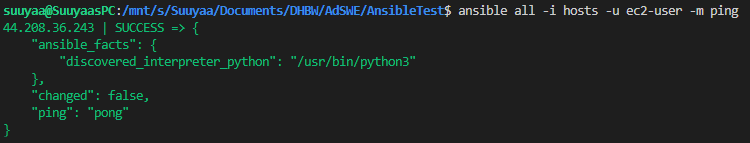
\includegraphics[width=12cm]{AnsibleScreenshots/adhoc.png}
    \caption{ad hoc Befehl in Ansible, zur Ausführung eines Pings auf ein angelegtes Hostsystem}
    \label{fig:adhoccommand}
\end{figure}\\
Da eine Automatisierung durch Ansible mit IaC ermöglicht werden soll, liegt das Hauptaugenmerk um Konfigurationen durchzuführen auf den Ansible-Playbooks. Diese führen verschiedene Tasks nacheinander aus. Sie werden durch den Befehl \textit{ansible-playbook -i [Zielinventory] [Playbook-Datei]} ausgeführt. An oberster Stelle eines Playbooks wird dessen Namen angegeben und zur Eingrenzung auf welchem Host und als welcher User dieses ausgeführt werden soll. In Listing \ref{lst:mariadbpb} ist eine solche Deklaration für ein Playbook zu sehen, welches für die Installation von MariaDB verantwortlich sein soll. 
\begin{lstlisting}[language=yaml, caption={Beschreibung eines Playbooks mit dem Namen \textit{mariadb test}}, label=lst:mariadbpb]
    ---
    - name: mariadb test #playbook
      hosts: TestServer #host name
      remote_user: ec2-user #remote user on host platform
      become: yes #root rights
\end{lstlisting}
% \begin{figure}
%     \centering
%     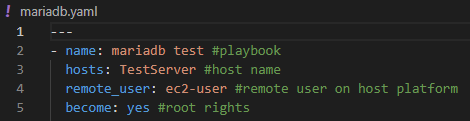
\includegraphics[width=12cm]{AnsibleScreenshots/mariadbpb.png}
%     \caption{Beschreibung eines Playbooks mit dem Namen \textit{mariadb test}}
%     \label{fig:mariadbpb}
% \end{figure}\\

Innerhalb dieses Playbooks können nun verschiedene Tasks angegeben werden. Diesen werden prozedural abgearbeitet. Des Weiteren können innerhalb des Playbooks verschiedene Variablen definiert werden, welche beispielsweise beim Ausführen des Playbooks zusammen mit dem Befehl angegeben werden können oder durch einen anderen Playbook Ablauf gesetzt werden. In Listing \ref{lst:mariadbtasks} ist zu erkennen, wie Tasks zum Installieren von MariaDB, dem anschließenden Erstellen einer zugehörigen conf-File, einer log-File und dem abschließenden Starten von MariaDB definiert sind. Ebenfalls anzumerken ist das Nutzen der Variable \textit{mysql\_port}. Diese wird in der Konfiguration Datei, welche als Template in Zeile 17 angegeben wird verwendet und kann somit angepasst werden. Des Weiteren wird in Zeile 18 ein \textit{notify} Befehl genutzt, welcher anhand des Namens innerhalb der Handler in Zeile 26 geregelt wird. Ein Notify-Befehl wird nur einmal ausgeführt, solange keine changes erfasst werden. Sollte sich das Playbook  in gewissen Maßen ändern, wird der Handler zum Neustarten nicht ausgeführt ein weiteres Mal durchgeführt. Ändert sich jedoch der Task \textit{create mysql configuration file}, also wird beispielsweise die \textit{mysql\_port}-Variable angepasst, so muss MariaDB neugestartet werden um weiterhin korrekt durchgeführt zu werden. Da sich die Datei \textit{src\_my.cnf.j2} nun verändert hat, bemerkt Ansible die Änderung und ein Change wird getriggert. Anhand des Changes wird nun der Notify Befehl ausgeführt und der Handler \textit{restart mariadb} startet den Service neu.  Des Weiteren kann innerhalb eines Tasks die Ausführung eines anderen Tasks inkludiert werden, indem mit \textit{include\_tasks: [Pfad zur Task-Datei]} eine Referenz auf den entsprechenden Task gesetzt wird (Zeile 11).
\begin{lstlisting}[language=yaml, caption={Beschreibung eines Playbooks mit dem Namen \textit{mariadb test}}, label=lst:mariadbtasks,firstnumber=7]
  vars:
    mysql_port: 3306

  tasks:
  - include_tasks: selinux.yaml #Putting the include at the top of tasks means it will be executed first
  # path: // Same direcotry, so no path is required
  - name: installing mariadb
    yum: name=mariadb-server state=latest

  - name: create mysql configuration file
    template: src=my.cnf.j2 dest=/etc/my.cnf
    notify: restart mariadb #triggers at end of task and only once (multiple notifies possible)

  - name: create mariadb log file
    file: path=/var/log/mysqld.log state=touch owner=mysql group=mysql mode=0775

  - name: start mariadb service
    service: name=mariadb state=started enabled=yes

  handlers: #handlers for notifies
  - name: restart mariadb
    service: name=mariadb state=restarted
#-include: selinux.yaml // Putting the include at the end of the file/top hierarchy executes the target as a standard playbook. That means e.g. conditionals or failtesting of this playbook won't apply on the included one.
\end{lstlisting}
% \pagebreak
% \begin{figure}
%     \centering
%     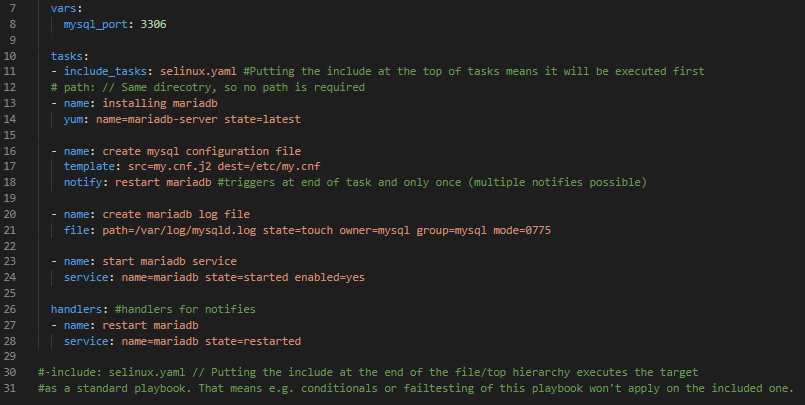
\includegraphics[width=12cm]{AnsibleScreenshots/mariadbtasks.png}
%     \caption{Beschreibung eines Playbooks mit dem Namen \textit{mariadb test}}
%     \label{fig:mariadbtasks}
% \end{figure}

Die Ausführung Tasks können wiederum anhand von Conditionals präziser geregelt werden. So kann die Ausführung eines Tasks beispielsweise auf eine Variable beschränkt werden oder anhand von weiteren Parametern wie dem Betriebssystem oder Error-Logs des Zielhosts ausgemacht werden (siehe Listing \ref{lst:conditionals}).
\begin{lstlisting}[language=yaml, caption={Das MariaDB Beispiel wird umgeben von einem Block, um ein Conditional auf alle Tasks zu beziehen}, label=lst:conditionals]
  vars:
    unicorn: true

  tasks:
  - name: don't install on debian machines
    yum: name=httpd state=latest #install httpd server
    when: (ansible_os_family=="RedHat" and ansible_distribution_major_version=="6") #condition on operating system

  - name: are unicorns real or fake
    shell: echo "unicorns are fake"
    when: not unicorn #unicorn variable is true, task will be skipped
\end{lstlisting}
% \begin{figure}
%     \centering
%     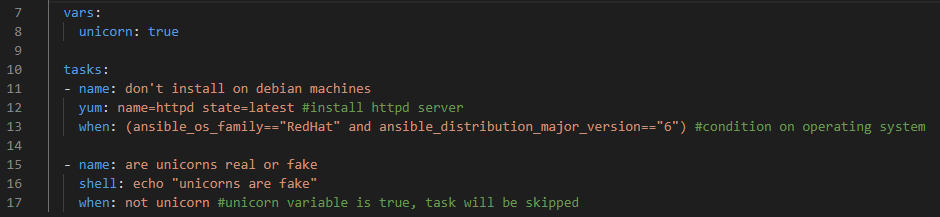
\includegraphics[width=12cm]{AnsibleScreenshots/conditionals.png}
%     \caption{Das MariaDB Beispiel wird umgeben von einem Block, um ein Conditional auf alle Tasks zu beziehen}
%     \label{fig:conditionals}
% \end{figure}

Um Tasks eine weitere Abstraktionsebene zu schaffen können diese in Blocks eingeteilt werden. Blöcke können beliebig in weitere Blocks unterteilt werden. Auf einen Block bezogen können anschließend wiederum Befehle ausgeführt. Vor allem Conditionals oder verschiedene Error-Handlings bieten hier einen Vorteil um eine Ansammlung an Tasks bedingt zu betrachten und auszuführen. Das Beispiel in Listing \ref{lst:blockandconditional} spiegelt das MariaDB Beispiel wieder, jedoch erfolgt die Installation ausschließlich unter der Bedingung, dass der Zielhost der Betriebssystem-Familie von \textit{"RedHat"} angehört (Zeile 25).
\begin{lstlisting}[language=yaml, caption={Das MariaDB Beispiel wird von einem Block umgeben, um ein Conditional auf alle enthaltenen Tasks zu beziehen}, label=lst:blockandconditional]
  tasks:
    - block:
        - name: installing mariadb
          yum: name=mariadb-server state=latest

        - name: create mysql configuration file
          template: src=my.cnf.j2 dest=/etc/my.cnf
          notify: restart mariadb #triggers at end of task and only once (multiple notifies possible)

        - name: create mariadb log file
          file: path=/var/log/mysqld.log state=touch owner=mysql group=mysql mode=0775

        - name: start mariadb service
          service: name=mariadb state=started enabled=yes

      when: ansible_os_family=="RedHat" #Conditional for whole block instead of each task
      become: yes
\end{lstlisting}
% \pagebreak
% \begin{figure}
%     \centering
%     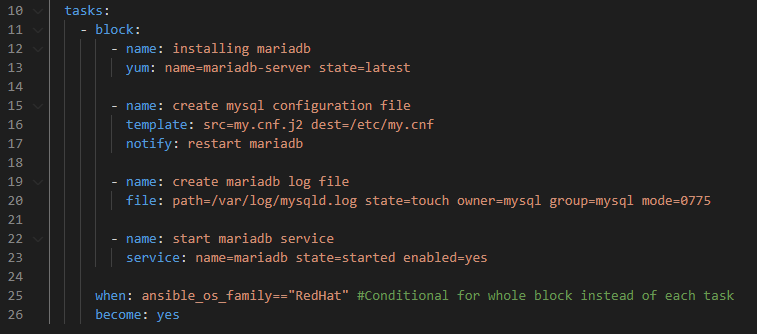
\includegraphics[width=12cm]{AnsibleScreenshots/block and conditional.png}
%     \caption{Das MariaDB Beispiel wird von einem Block umgeben, um ein Conditional auf alle enthaltenen Tasks zu beziehen}
%     \label{fig:blockandconditional}
% \end{figure}

Eine Weitere Möglichkeit um ein Ansible Projekt weitergehend zu abstrahieren und strukturieren wird durch Roles bereitgestellt. Diese können über eine Ansible-Galaxy erstellt werden. Eine neue Rolle kann durch den Befehl \textit{ansible-galaxy init [Role-Name]} erstellt werden. Ein großer Vorteil von Ansible-Galaxies ist die Verfügbarkeit von diversen Community-Galaxies. So kann auf \url{https://galaxy.ansible.com/} nach verschiedenen von Anwendern erstellten Rollen gesucht werden, welche durch vorgefertigte Konfigurationen eine Verwaltung bestimmter Systeme erlauben und frei erweitert werden können.\\
Das Erstellen einer Rolle kann vereinfacht als eine Unterteilung des Playbooks in verschiedene Bereiche betrachtet werden. Eine Rolle kann anschließend über ein übliches Ansible-Playbook gestartet werden (siehe Listing \ref{lst:startroles}).
\begin{lstlisting}[language=yaml, caption={Ein Playbook zum Ausführen der Rollen} \textit{common} und \textit{roles\_example}, label=lst:startroles]
    ---
    - name: deploy common and mariadb role
      hosts: TestServer
      remote_user: ec2-user
      become: yes
    
      roles:
      - common
      - roles_example
\end{lstlisting}
%\pagebreak
% \begin{figure}
%     \centering
%     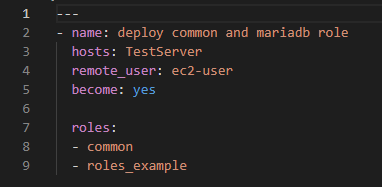
\includegraphics[width=8cm]{AnsibleScreenshots/call role.png}
%     \caption{Ein Playbook zum Ausführen der Rollen} \textit{common} und \textit{roles\_example}
%     \label{fig:startroles}
% \end{figure}

Innerhalb des Role-Directories bestehen nun verschiedene Directories für die jeweiligen Bestandteile eines Playbooks. Diese sind wie folgt.
\begin{itemize}
    \item \textit{tasks}, zur Definition der verschiedenen Tasks.
    \item \textit{handlers}, zur Definition verschiedener Handler.
    \item \textit{vars}, zur Definition verschiedener Variablen.
    \item \textit{defaults}, zur Definition von Standardwerten, sollten Variablen nicht explizit gesetzt sein.
    \item \textit{templates}, zum Anlegen verschiedener Dateien, welche als Vorlage dienen.
    \item \textit{meta}, zum Definieren verschieder Metadaten der Rolle. Eine nützliche Funktion hierbei ist das Definieren verschiedener Role Dependencies. Diese binden die Rolle und deren Tasks an die entsprechende Definition, wodurch z.B. eine Rolle auf alle Zielsysteme angewandt werden kann, solange diese mit einem bestimmten Betriebssystem ausgeführt werden (siehe Listing \ref{lst:roledependency}).
\end{itemize}
\begin{lstlisting}[language=yaml, caption={Ausschnitt der \textit{main.yaml} des \textit{meta}-Directories, welche eine Role Dependency definiert}, label=lst:roledependency]
    dependencies: 
      - {role: apache, when: "ansible_os_family=='RedHat'"} #Depend on Apache role, if our host is of OS type RedHat
\end{lstlisting}
% \begin{figure}%     \centering
%     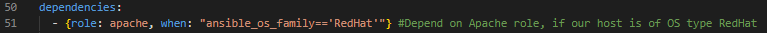
\includegraphics[width=12cm]{AnsibleScreenshots/role dependency.png}
%     \caption{Ausschnitt der \textit{main.yaml} des \textit{meta}-Directories, welche eine Role Dependency definiert.}
%     \label{fig:roledependency}
% \end{figure}\\

Eine weitere Funktion von Ansible, welche diese Arbeit abschließen soll, ist die Möglichkeit ein Error-Handling innerhalb der Tasks zu betreiben. Da ein Ansible Playbook unterbrochen wird, sobald ein Fehler bei dessen Ausführung auftritt, ist ein geeignetes Error-Handling von Vorteil, um ungewollte Abläufe innerhalb der Automatisierung zu verhindern. Hierbei sind vor allem die Befehle \textit{ignore\_error}, welcher die Auführung des Playbooks trotz eines Errors fortführt und \textit{failed\_when}, welcher einen Error anhand einer Bedingung erzeugt. Des Weiteren kann mit Hilfe des \textit{changed\_when} Befehls ein \textit{changed}-Event in einen erfolgreichen \textit{ok}-Event, anhand einer Bedingung umgewandelt werden. So kann z.B. eine Änderung der conf-File (siehe Listing \ref{lst:mariadbtasks}) ignoriert werden, um den \textit{notify}-Befehl zu überspringen. Ein Beispiel zum Error-Handling ist in Listing \ref{lst:error-handling} zu sehen.
\begin{lstlisting}[language=yaml, caption={Ansible Beispiel Task mit Error-Handling}, label=lst:error-handling]
    ---
    - name: testing error handling
      hosts: TestServer
      remote_user: ec2-user
      become: yes
    
      tasks:
      - name: testing ignore errors
        user: name=Max password={{uPassword}}
        ignore_errors: yes
    
      - name: next task
        shell: echo hello world
    
      - name: quick echo
        shell: echo $PATH
        register: result
        changed_when: false #results in "ok" on change
    
      - debug: msg="Stop running playbook if the play failed"
        failed_when: result is failed
    
      - name: echo failed #doesnt actually fail
        shell: echo I failed
        register: output
    
      - debug: msg="Okay really stop the playbook this time"
        failed_when: output.stdout.find("failed") != -1
    
      - name: just adding another task in here to show you that it will stop
        shell: echo hello world
\end{lstlisting}

% \pagebreak
% \begin{figure}
%     \centering
%     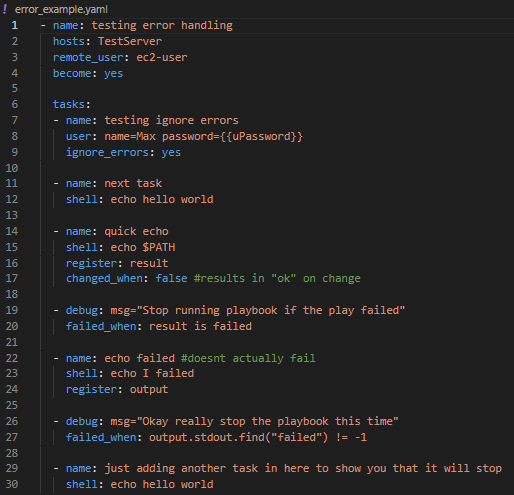
\includegraphics[width=12cm]{AnsibleScreenshots/error-handling.png}
%     \caption{Ansible Beispiel Task mit Error-Handling.}
%     \label{fig:error-handling}
% \end{figure}\\
%%% Angabe der .bib-Datei (ohne Endung) / State .bib file (for BibTeX usage)
\newpage
\printbibliography %\printbibliography if you use biblatex/Biber
\end{document}